\section{Multi-Assignment Clustering}

\subsection{Role-Based Access Control (RBAC)}
Given a \emph{user-permission} matrix $X\in \mathbb B^{D\times N}$, find
\begin{description}
\item[Roles] $U\in \mathbb B^{D\times K}$ and
\item[Assignments] $Z\in \mathbb B^{K\times N}$ 
\end{description}
with $\mathbb B=\{0,1\}$ such that
\begin{align*}
    X = U \otimes Z \quad \Leftrightarrow \quad x_{dn} = \bigvee_k [u_{dk} \land z_{kn}].
\end{align*}
\begin{itemize}
\item Each role defines a set of permissions
\item Users are assigned to a set of roles and get all permissions of these roles.
\end{itemize}

\subsubsection{Notation}
\begin{itemize}
\item $x_{dn} \in \{0,1\}$: Assignment of user $n$ to permission $d$.
\item $z_{kn} \in \{0,1\}$: Assignment of user $n$ to role $k$.
\item $u_{dk} \in \{0,1\}$: Assignment of permission $d$ to role $k$.
\item $\beta_{dk} \in [0,1]$: Probability of $u_{dk} = 0$.
\end{itemize}
\begin{figure}[H]
    \centering
    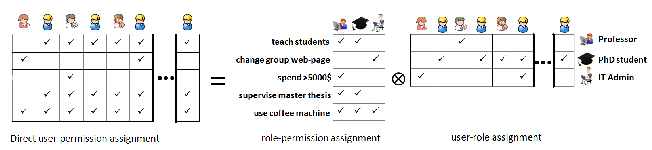
\includegraphics[width=\textwidth]{img/multi_assignment_rbac}
\end{figure}

\subsubsection{Evaluation Criteria}
For each role mining problem definition, there is a (set of) evaluation criteria:
\begin{itemize}
\item Matrix Reconstruction
\item Number of Sources
\item Inference Quality
\item Generalisation
\item 
\end{itemize}

\subsection{Binary Matrix Factorisation}
\emph{Min-Noise Approximation}: Given $K$, find the matrices $\hat U$, $\hat Z$ such that
\begin{align*}
    (\hat U, \hat Z) =\argmin_{U,Z} \norm{X-U\otimes Z}_1
\end{align*}
with $U\in \mathbb B^{D\times K}$ and $Z\in \mathbb B^{K\times N}$. This problem is also called \emph{approximate Boolean Matrix decomposition} and has the following properties:
\begin{itemize}
    \item \textbf{All} matrices are Boolean,
    \item It is a \emph{combinatorial optimisation problem},
    \item It is proven to be \emph{NP-hard} (reducible to set basis problem).
\end{itemize}
In contrast to recommender systems a the outputs $\hat U$ and $\hat Z$ are always binary.


